\documentclass[12pt,UTF8]{ctexart}
\usepackage{ctex,amsmath,amssymb,geometry,fancyhdr,bm,amsfonts
,mathtools,extarrows,graphicx,url,enumerate,color,float,multicol} 
% 加入中文支持
\newcommand\Set[2]{%
\left\{#1\ \middle\vert\ #2 \right\}}
\geometry{a4paper,scale=0.80}
\pagestyle{fancy}
\rhead{第7章补充题}
\lhead{基础习题课讲义}
\chead{微积分B(1)}
\begin{document}
\def\thesection{11C}
\section{第7章补充题}
\def\thesubsection{\thesection.\arabic{subsection}}
\subsection{第7章补充题解答}
\begin{enumerate}
\item设$f\in R[a,b],g\in R[a,b]$,求证:
\[
\Big(\int_a^bf(x)g(x)\mathrm dx\Big)^2\leq\int_a^bf^2(x)\mathrm dx\int_a^bg^2(x)\mathrm dx
\]
证明:令$F(x)=\Big(\int_a^xf(t)g(t)\mathrm dt\Big)^2-\int_a^xf^2(t)\mathrm dt\int_a^xg^2(t)\mathrm dt$

$F'(x)=2\int_a^xf(t)g(t)\mathrm dtf(x)g(x)-f^2(x)\int_a^xg^2(t)\mathrm dt-g^2(x)\int_a^xf^2(t)\mathrm dt\\
=\int_a^x[2f(t)g(t)f(x)g(x)-f^2(x)g^2(t)-g^2(x)f^2(t)]\mathrm dt\\
=-\int_a^x[f(x)g(t)-f(t)g(x)]^2\mathrm dt\leq0$

$\therefore F(x)\leq F(0)=0$,即$\Big(\int_a^bf(x)g(x)\mathrm dx\Big)^2\leq\int_a^bf^2(x)\mathrm dx\int_a^bg^2(x)\mathrm dx$.

\item设$f(x)$在区间$[0,1]$上连续且单调减少,又设$f(x)>0$,求证对于任意满足$0<\alpha<\beta<1$的$\alpha$和$\beta$,有
\[
\beta\int_0^\alpha f(x)\mathrm dx>\alpha\int_0^\beta f(x)\mathrm dx
\]
证明:方法1:令$F(x)=x\int_0^\alpha f(t)\mathrm dt-\alpha\int_0^xf(t)\mathrm dt$

$F'(x)=\int_0^\alpha f(t)\mathrm dt-\alpha f(x),F''(x)=-\alpha f'(x)$

$\because f(x)$在区间$[0,1]$上连续且单调减少

$\therefore F''(x)=-\alpha f'(x)>0$

$\therefore$当$x>\alpha$时$F'(x)=\int_0^\alpha f(t)\mathrm dt-\alpha f(x)>F(\alpha)=\int_0^\alpha f(t)\mathrm dt-\alpha f(\alpha)\\
=\int_0^\alpha[f(t)-f(\alpha)]\mathrm dt>0$

$\therefore$当$x>\alpha$时$F(x)>F(\alpha)=0$

$\therefore$对于任意满足$0<\alpha<\beta<1$的$\alpha$和$\beta$,有$\beta\int_0^\alpha f(x)\mathrm dx>\alpha\int_0^\beta f(x)\mathrm dx$.

方法2:$\beta\int_0^\alpha f(x)\mathrm dx-\alpha\int_0^\beta f(x)\mathrm dx=\beta\int_0^\alpha f(x)\mathrm dx-\alpha\int_0^\alpha f(x)\mathrm dx-\alpha\int_\alpha^\beta f(x)\mathrm dx\\
=(\beta-\alpha)\int_0^\alpha f(x)\mathrm dx-\alpha\int_\alpha^\beta f(x)\mathrm dx=(\beta-\alpha)\alpha f(\xi_1)-\alpha(\beta-\alpha)f(\xi_2)\\
=\alpha(\beta-\alpha)[f(\xi_1)-f(\xi_2)]>0,\xi_1\in(0,\alpha),\xi_2\in(\alpha,\beta)$

$\therefore$对于任意满足$0<\alpha<\beta<1$的$\alpha$和$\beta$,有$\beta\int_0^\alpha f(x)\mathrm dx>\alpha\int_0^\beta f(x)\mathrm dx$.

\item设$f(x),g(x)$在区间$[0,+\infty)$上连续,其中$f(x)>0(0\leq x<+\infty)$,$g(x)$在区间$[0,+\infty)$上单调增加,令
\[
\varphi(x)=\frac{\int_0^xf(t)g(t)\mathrm dt}{\int_0^xf(t)\mathrm dt}.
\]
求证$\varphi(x)$在区间$[0,+\infty)$上单调增加.

证明:$\because f(x)>0(0\leq x<+\infty)$,$g(x)$在区间$[0,+\infty)$上单调增加

$\therefore\varphi'(x)=\frac{f(x)g(x)\int_0^xf(t)\mathrm dt-f(x)\int_0^xf(t)g(t)\mathrm dt}{[\int_0^xf(t)\mathrm dt]^2}=f(x)\frac{\int_0^xf(t)[g(x)-g(t)]\mathrm dt}{[\int_0^xf(t)\mathrm dt]^2}>0,x\in[0,+\infty)$

【或者$\varphi'(x)=\frac{f(x)g(x)\int_0^xf(t)\mathrm dt-f(x)\int_0^xf(t)g(t)\mathrm dt}{[\int_0^xf(t)\mathrm dt]^2}=f(x)\frac{\int_0^xf(t)[g(x)-g(t)]\mathrm dt}{[\int_0^xf(t)\mathrm dt]^2}\\
=f(x)\frac{xf(\xi)[g(x)-g(\xi)]}{[\int_0^xf(t)\mathrm dt]^2}>0,\xi\in(0,x),x\in[0,+\infty)$】

$\therefore\varphi(x)$在区间$[0,+\infty)$上单调增加.
\item设$f'(x)$在区间$[a,b]$上连续,且$f(a)=f(b)=0$,求证:
\[
\Big|\int_a^bf(x)\mathrm dx\Big|\leq\frac{(b-a)^2}4\max\limits_{a\leq x\leq b}|f'(x)|
\]
证明:$\because f'(x)$在区间$[a,b]$上连续,且$f(a)=f(b)=0$

$\therefore f(x)=f'(\xi_1)(x-a),f(x)=f'(\xi_2)(x-b),\xi_1\in(a,x),\xi_2\in(x,b)$

$\therefore\big|\int_a^{\frac{a+b}2}f(x)\mathrm dx\big|=\big|\int_a^{\frac{a+b}2}f'(\xi_1)(x-a)\mathrm dx\big|\leq\int_a^{\frac{a+b}2}\big|f'(\xi_1)\big|(x-a)\mathrm dx\\
\leq\int_a^{\frac{a+b}2}\max\limits_{a\leq x\leq b}\big|f'(x)\big|(x-a)\mathrm dx=\max\limits_{a\leq x\leq b}\big|f'(x)\big|\int_a^{\frac{a+b}2}(x-a)\mathrm dx=\frac18(b-a)^2\max\limits_{a\leq x\leq b}\big|f'(x)\big|$

$\big|\int_{\frac{a+b}2}^bf(x)\mathrm dx\big|=\big|\int_{\frac{a+b}2}^bf'(\xi_2)(x-b)\mathrm dx\big|\leq\int_{\frac{a+b}2}^b\big|f'(x)\big|(b-x)\mathrm dx\\
\leq\int_{\frac{a+b}2}^b\max\limits_{a\leq x\leq b}\big|f'(x)\big|(b-x)\mathrm dx=\max\limits_{a\leq x\leq b}\big|f'(x)\big|\int_{\frac{a+b}2}^b(b-x)\mathrm dx=\frac18(b-a)^2\max\limits_{a\leq x\leq b}\big|f'(x)\big|$

$\therefore\big|\int_a^bf(x)\mathrm dx\big|=\big|\int_a^{\frac{a+b}2}f(x)\mathrm dx+\int_{\frac{a+b}2}^bf(x)\mathrm dx\big|\leq\big|\int_a^{\frac{a+b}2}f(x)\mathrm dx\big|+\big|\int_{\frac{a+b}2}^bf(x)\mathrm dx\big|\\
\leq\frac18(b-a)^2\max\limits_{a\leq x\leq b}\big|f'(x)\big|+\frac18(b-a)^2\max\limits_{a\leq x\leq b}\big|f'(x)\big|=\frac14(b-a)^2\max\limits_{a\leq x\leq b}\big|f'(x)\big|$.

\item设$f(x)$在区间$[a,b]$上连续且单调增加,证明:
\[
\int_a^bxf(x)\mathrm dx\geq\frac{a+b}2\int_a^bf(x)\mathrm dx
\]
证明:$\int_a^b(x-\frac{a+b}2)f(x)\mathrm dx=\int_a^{\frac{a+b}2}(x-\frac{a+b}2)f(x)\mathrm dx+\int_{\frac{a+b}2}^b(x-\frac{a+b}2)f(x)\mathrm dx$

$\because f(x)$在$[a,b]$上连续,$g(x)=x-\frac{a+b}2$在$[a,\frac{a+b}2]$上连续且非正,$g(x)=x-\frac{a+b}2$在$[\frac{a+b}2,b]$上连续且非负

$\therefore\int_a^b(x-\frac{a+b}2)f(x)\mathrm dx=f(\xi_1)\int_a^{\frac{a+b}2}(x-\frac{a+b}2)\mathrm dx+f(\xi_2)\int_{\frac{a+b}2}^b(x-\frac{a+b}2)\mathrm dx\\
=f(\xi_1)(\frac12x^2-\frac{a+b}2x)\Big|_a^{\frac{a+b}2}+f(\xi_2)(\frac12x^2-\frac{a+b}2x)\Big|_{\frac{a+b}2}^b\\
=\frac18(b-a)^2[f(\xi_2)-f(\xi_1)],\xi_2\in(\frac{a+b}2,b),\xi_1\in(a,\frac{a+b}2)$

$\because f(x)$在$[a,b]$上单调增加

$\therefore\int_a^b(x-\frac{a+b}2)f(x)\mathrm dx=\frac18(b-a)^2[f(\xi_2)-f(\xi_1)]>0$,即$\int_a^bxf(x)\mathrm dx\geq\frac{a+b}2\int_a^bf(x)\mathrm dx$.

\item设$f(x)$在区间$[0,1]$上连续,下凸且非负,$f(0)=0$,求证:
\[
\int_0^{\frac12}f(x)\mathrm dx\leq\frac14\int_0^1f(x)\mathrm dx.
\]
证明:$\because f(x)$下凸

$\therefore\forall x_1,x_2\in[0,1]$有$f(\frac{x_1+x_2}2)\leq\frac12[f(x_1)+f(x_2)]$

$\therefore\int_0^{\frac12}f(x)\mathrm dx=\frac12\int_0^1f(\frac u2)\mathrm du=\frac12\int_0^1f(\frac{u+0}2)\mathrm du\leq\frac12\int_0^1\frac12[f(u)+f(0)]\mathrm du=\frac14\int_0^1f(u)\mathrm du\\
=\frac14\int_0^1f(x)\mathrm dx$.

\item设$f(x)$在区间$[a,b]$上连续且$f(x)\geq0$,又令$M=\max\limits_{a\leq x\leq b}\{f(x)\}$,求证:
\[
\lim\limits_{n\rightarrow\infty}\Big(\int_a^bf^n(x)\mathrm dx\Big)^{\frac1n}=M.
\]
证明:记$f(x_0)=M=\max\limits_{a\leq x\leq b}\{f(x)\}$

$\because f(x)$在区间$[a,b]$上连续

$\therefore\forall\varepsilon>0$且$\varepsilon<M$存在$x_0$的邻域$I\subset[a,b],s.t.f(x)>M-\varepsilon>0,x\in I$

$\therefore M=(M^n)^{\frac1n}=\Big(\int_a^bM^n\mathrm dx\Big)^{\frac1n}\geq\Big(\int_a^bf^n(x)\mathrm dx\Big)^{\frac1n}\geq\Big(\int_If^n(x)\mathrm dx\Big)^{\frac1n}\\
>\Big(\int_I(M-\varepsilon)^n\mathrm dx\Big)^{\frac1n}=(M-\varepsilon)\Big(\int_I\mathrm dx\Big)^{\frac1n}=M-\varepsilon$

$\therefore-\varepsilon<\Big(\int_a^bf^n(x)\mathrm dx\Big)^{\frac1n}-M<0<\varepsilon$

$\therefore\lim\limits_{n\rightarrow\infty}\Big(\int_a^bf^n(x)\mathrm dx\Big)^{\frac1n}=M$.

\item设$f\in C[a,b]$,如果对于任意一个满足$g(a)=g(b)=0$的$g\in C[a,b]$,都有$\int_a^bf(x)g(x)\mathrm dx=0$. 求证:$f(x)\equiv0$.

证明:假设$\exists x_0\in[a,b],s.t.f(x_0)\neq0$. 不妨设$x_0\in(a,b),f(x_0)>0$. 这时存在包含$x_0$的区间$[x_1,x_2]\subset[a,b]$,使得$\forall x\in[x_1,x_2]$,有$f(x)>0$. 构造函数
\[
g(x)=\begin{cases}
(x-x_1)^2(x-x_2)^2,&x_1<x<x_2,\\
0,&\text{otherwise}.
\end{cases}
\]
则有$\int_a^bf(x)g(x)\mathrm dx=\int_{x_1}^{x_2}f(x)g(x)\mathrm dx=f(\xi)\int_{x_1}^{x_2}g(x)\mathrm dx>0$. 这与对于任意一个满足$g(a)=g(b)=0$的$g\in C[a,b]$,都有$\int_a^bf(x)g(x)\mathrm dx=0$矛盾.

故$f(x)\equiv0$.

\item设$f\in C(0,+\infty)$,并且对任意的$a>0$和$b>1$,积分值$\int_a^{ab}f(x)\mathrm dx$与$a$无关. 求证:存在常数$c$使得$f(x)=\frac cx$.

证明:令$F(a)=\int_a^{ab}f(x)\mathrm dx,a>0,b>10$

$\because$对任意的$a>0$和$b>1$,积分值$\int_a^{ab}f(x)\mathrm dx$与$a$无关

$\therefore\frac{\mathrm dF}{\mathrm da}=bf(ab)-f(a)\equiv0$

取$a=1$,则$bf(b)=f(1),f(b)=\frac{f(1)}b,b>1$

$\because f\in C(0,+\infty)$

$\therefore f(b)=\frac{f(1)}b$在$b=1$时也成立

即$f(x)=\frac cx,x\geq1,c=f(1)$

当$0<b<1$时,$\int_1^bf(x)\mathrm dx\xlongequal{u=\frac1x}-\int_{\frac1b}^1f(\frac1u)\frac1{u^2}\mathrm du=\int_1^{\frac1b}f(\frac1u)\frac1{u^2}\mathrm du=\int_1^{\frac1b}\frac c{\frac1u}\frac1{u^2}\mathrm du\\
=c\int_1^{\frac1b}\frac1u\mathrm du=-c\ln b$

两端对$b$求导,得到$f(b)=\frac cb,0<b<1$,即$\forall x\in(0,1),f(x)=\frac cx$

综上所述:$f(x)=\frac cx,x\in(0,+\infty)$.
\item设$f\in R[a,b]$,其中$b-a=1$,求证:
\\
(1)$\mathrm e^{\int_a^bf(x)\mathrm dx}\leq\int_a^b\mathrm e^{f(x)}\mathrm dx$;\\
(2)若$f(x)\geq c>0$,则$\int_0^1\ln f(x)\mathrm dx\leq\ln\int_0^1f(x)\mathrm dx$.

证明:(1)记$T:a=x_0<x_1<x_2<\cdots<x_n=b$为区间$[a,b]$的一个分割,则$\int_a^bf(x)\mathrm dx=\lim\limits_{\lambda\rightarrow0}f(\xi_i)\Delta x_i,\Delta x_i=x_i-x_{i-1},\xi\in(x_{i-1},x_i)$

$\because g(x)=\mathrm e^x$下凸

故
\[\begin{split}
\mathrm e^{\frac{\Delta x_1}{b-a}f(\xi_1)+\frac{\Delta x_2}{b-a}f(\xi_2)+\cdots+\frac{\Delta x_n}{b-a}f(\xi_n)}=&\mathrm e^{\Delta x_1f(\xi_1)+\Delta x_2f(\xi_2)+\cdots+\Delta x_nf(\xi_n)}\\
\leq&\Delta x_1\mathrm e^{f(\xi_1)}+\Delta x_2\mathrm e^{f(\xi_2)}+\cdots+\Delta x_n\mathrm e^{f(\xi_n)}\end{split}\]即$\mathrm e^{\sum_{i=1}^n\Delta x_if(\xi_i)}\leq\sum_{i=1}^n\mathrm e^{f(\xi_i)}\Delta x_i$,两边取极限得
\[
\mathrm e^{\int_a^bf(x)\mathrm dx}=\lim\limits_{\lambda\rightarrow0}\mathrm e^{\sum_{i=1}^n\Delta x_if(\xi_i)}\leq\lim\limits_{\lambda\rightarrow0}\sum_{i=1}^n\mathrm e^{f(\xi_i)}\Delta x_i=\int_a^b\mathrm e^{f(x)}\mathrm dx.
\]

(2)$\because h(x)=\ln x$上凸

$\therefore$对于区间$[0,1]$的分割$T^*:0=x_0<x_1<x_2<\cdots<x_n=1,\Delta x_i=x_i-x_{i-1},\eta_i\in(x_{i-1},x_i)$
\[\begin{split}
&\ln[\frac{\Delta x_1}{1-0}f(\eta_1)+\frac{\Delta x_2}{1-0}f(\eta_2)+\cdots+\frac{\Delta x_n}{1-0}f(\eta_n)]\\
=&\ln[\Delta x_1f(\eta_1)+\Delta x_2f(\eta_2)+\cdots+\Delta x_nf(\eta_n)]\\
\geq&\Delta x_1\ln f(\eta_1)+\Delta x_2\ln f(\eta_2)+\cdots+\Delta x_nf(\eta_n)
\end{split}\]
即$\ln[\sum_{i=1}^n\Delta x_if(\eta_i)]\geq\sum_{i=1}^n\Delta x_i\ln f(\eta_i)$,两边取极限得
\[
\ln\int_0^1f(x)\mathrm dx=\lim\limits_{\lambda\rightarrow0}\ln[\sum_{i=1}^n\Delta x_if(\eta_i)]\geq\lim\limits_{\lambda\rightarrow0}\sum_{i=1}^n\Delta x_i\ln f(\eta_i)=\int_0^1\ln f(x)\mathrm dx
\]

即$\int_0^1\ln f(x)\mathrm dx\leq\ln\int_0^1f(x)\mathrm dx$.

\item设$f\in C[0,\pi]$,求证:
\[
\lim\limits_{n\rightarrow\infty}\int_0^{\pi}f(x)|\sin nx|\mathrm dx=\frac2\pi\int_0^\pi f(x)\mathrm dx.
\]

{\bf【注意:原题给的条件为$f\in R[0,\pi]$,这里改成了$f\in C[0,\pi]$,以便应用推广的积分中值定理。】}

证明:$\int_0^\pi f(x)|\sin nx|\mathrm dx=\sum_{k=1}^n\int_{\frac{k-1}n\pi}^{\frac kn\pi}f(x)|\sin nx|\mathrm dx$

$\because f(x)\in C[0,\pi],g(x)=|\sin nx|$在$[\frac{k-1}n\pi,\frac kn\pi]$上连续且非负

$\therefore$根据推广的积分中值定理
\[\int_{\frac{k-1}n\pi}^{\frac kn\pi}f(x)|\sin nx|\mathrm dx=f(\xi_k)\int_{\frac{k-1}n\pi}^{\frac kn\pi}|\sin nx|\mathrm dx=\frac2nf(\xi_k),\xi_k\in(\frac kn\pi,\frac{k-1}n\pi)\]
$\therefore\int_0^\pi f(x)|\sin nx|\mathrm dx=\sum_{k=1}^n\frac2nf(\xi_k)=\frac2\pi\sum_{k=1}^nf(\xi_k)\frac\pi n$

$\therefore\lim\limits_{n\rightarrow\infty}\int_0^{\pi}f(x)|\sin nx|\mathrm dx=\lim\limits_{n\rightarrow\infty}\frac2\pi\sum_{k=1}^nf(\xi_k)\frac\pi n=\frac2\pi\int_0^\pi f(x)\mathrm dx$.
\item若$f$为连续函数,求证:
\[
\int_0^xf(u)(x-u)\mathrm du=\int_0^x\big(\int_0^uf(t)\mathrm dt\big)\mathrm du.
\]
证明:$\int_0^xf(u)(u-x)\mathrm du=\int_0^x(u-x)\mathrm d[\int_0^uf(t)\mathrm dt]=(u-x)\int_0^uf(t)\mathrm dt\Big|_0^x-\int_0^x\big(\int_0^uf(t)\mathrm dt\big)\mathrm du\\
=-\int_0^x\big(\int_0^uf(t)\mathrm dt\big)\mathrm du$

$\therefore\int_0^xf(u)(x-u)\mathrm du=\int_0^x\big(\int_0^uf(t)\mathrm dt\big)\mathrm du$.
\item设$f(x)$在区间$[0,+\infty)$上一致连续且非负,如果无穷积分$\int_0^{+\infty}f(x)\mathrm dx$收敛,\\求证:$\lim\limits_{x\rightarrow+\infty}f(x)=0$.

证明:假设$\lim\limits_{x\rightarrow+\infty}f(x)\neq0$,则$\exists\varepsilon_0=2a>0,\forall X>0$,当$x>X$时,\\$|f(x)-0|=f(x)>\varepsilon_0=2a$

可取一单调增加且趋于$+\infty$的点列$\{x_n\},s.t.f(x_n)\geq2a,x_{n+1}-x_n>1,x_1>1$

$\because f(x)$在区间$[0,+\infty)$上一致连续

$\therefore$对于$\varepsilon_1=a>0,\exists b>0$(不妨设$b<\frac12$),当$|x-x_n|<b$时,$|f(x)-f(x_n)|<\varepsilon_1=a$

此时$f(x)-f(x_n)>-a,f(x)>f(x_n)-a\geq a$

则$\int_0^{x_{n+1}}f(x)\mathrm dx\geq\sum_{k=1}^n\int_{x_k-b}^{x_k+b}f(x)\mathrm dx\geq\sum_{k=1}^n\int_{x_k-b}^{x_k+b}a\mathrm dx=n\cdot a\cdot2b\rightarrow+\infty,n\rightarrow\infty$

$\therefore\lim\limits_{A\rightarrow+\infty}\int_0^Af(x)\mathrm dx=+\infty,\int_0^{+\infty}f(x)\mathrm dx$发散,假设不成立

$\therefore\lim\limits_{x\rightarrow+\infty}f(x)=0$.
\item计算两椭圆$\frac{x^2}{a^2}+\frac{y^2}{b^2}\leq1$和$\frac{x^2}{b^2}+\frac{y^2}{a^2}\leq1(a>0,b>0)$公共部分的面积.

解:由$\begin{cases}
\frac{x^2}{a^2}+\frac{y^2}{b^2}=1\\
\frac{x^2}{b^2}+\frac{y^2}{a^2}=1
\end{cases}$得两椭圆在第一象限的交点为$P(\frac{ab}{\sqrt{a^2+b^2}},\frac{ab}{\sqrt{a^2+b^2}})$
\begin{figure}[H]
\begin{center}
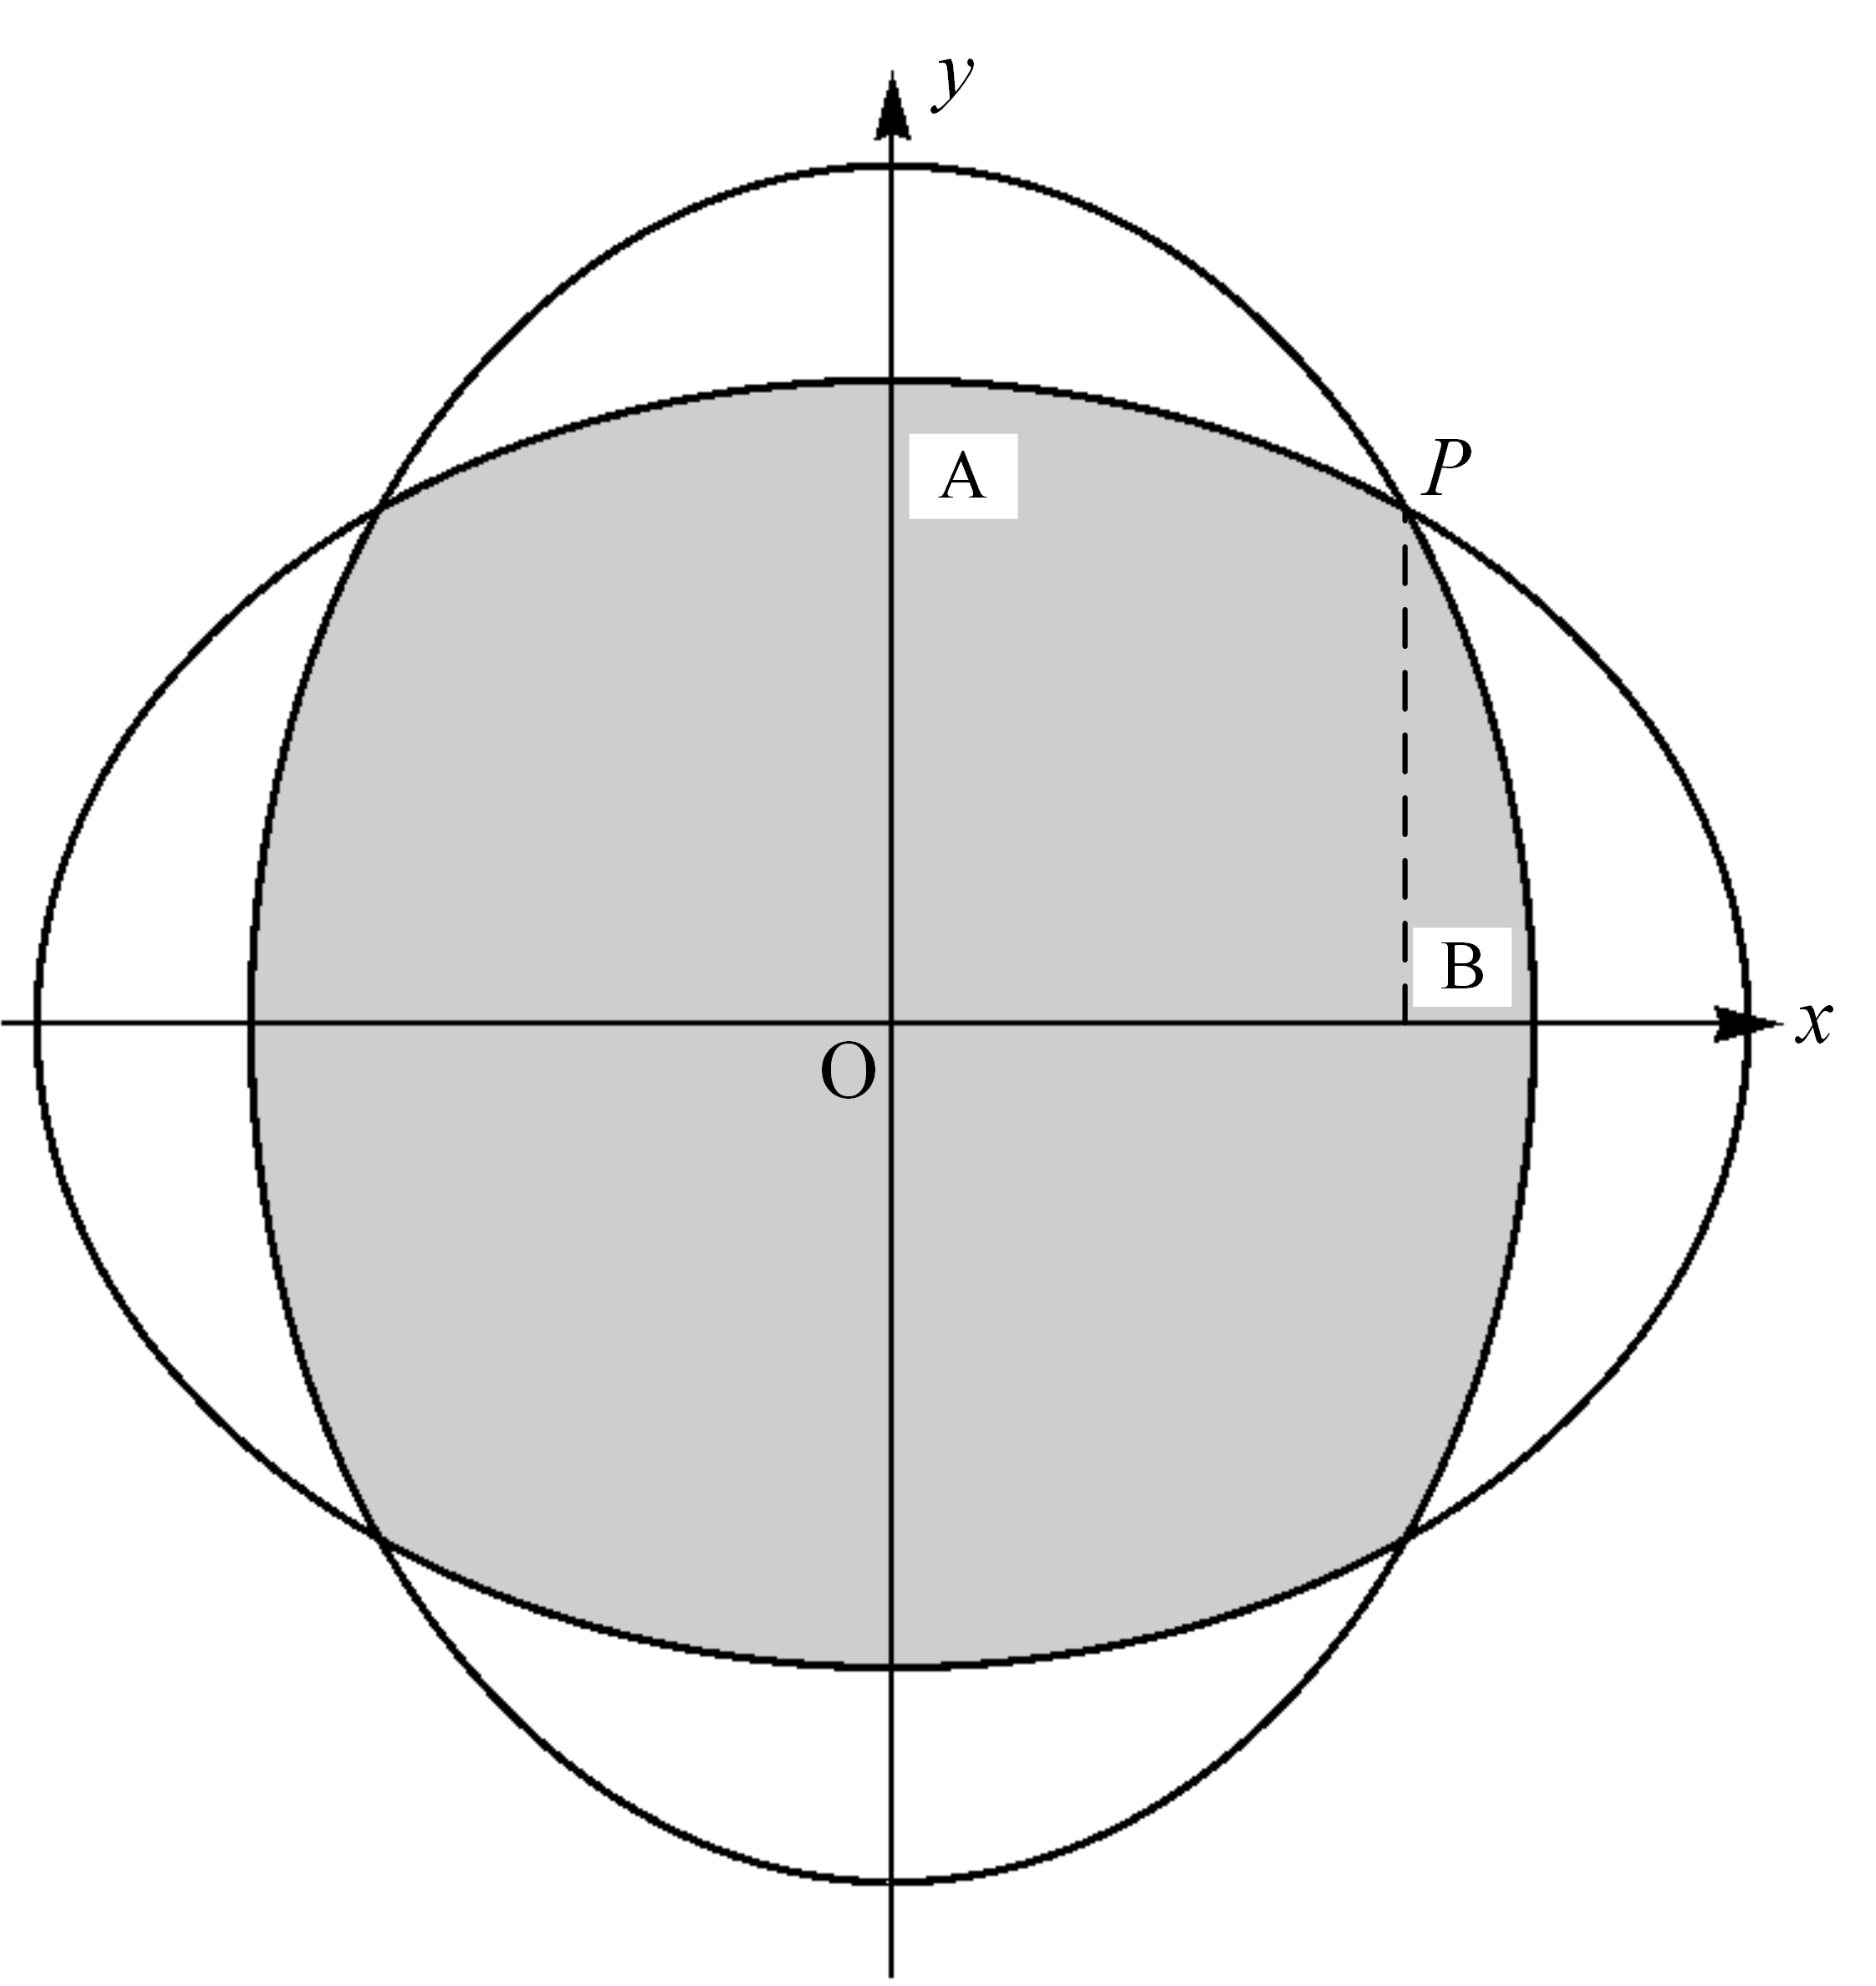
\includegraphics[height=0.4\textheight]{F:/life/2018AutumnTA/Exercises/11CExtra/Fig14.png}
\end{center}
\caption{第7章补充题 14题图示}
\label{14}
\end{figure}
如图\ref{14}所示,图形在第一象限内可以分成A,B两部分.

A部分的面积$S_A=\int_0^{\frac{ab}{\sqrt{a^2+b^2}}}y\mathrm dx=\int_0^{\frac{ab}{\sqrt{a^2+b^2}}}b\sqrt{1-\frac{x^2}{a^2}}\mathrm dx\\
\xlongequal{x=a\sin t}\int_0^{\arcsin\frac b{\sqrt{a^2+b^2}}}b\cos t\cdot a\cos t\mathrm dt=ab\int_0^{\arcsin\frac b{\sqrt{a^2+b^2}}}\cos^2t\mathrm dt\\
=ab\int_0^{\arcsin\frac b{\sqrt{a^2+b^2}}}\frac12(1+\cos2t)\mathrm dt=\frac{ab}2(t+\frac12\sin2t)\Big|_0^{\arcsin\frac b{\sqrt{a^2+b^2}}}\\
=\frac{ab}2(t+\sin t\sqrt{1-\sin^2t})\Big|_0^{\arcsin\frac b{\sqrt{a^2+b^2}}}=\frac{ab}2(\arcsin\frac b{\sqrt{a^2+b^2}}+\frac b{\sqrt{a^2+b^2}}\sqrt{1-\frac{b^2}{a^2+b^2}})\\
=\frac{ab}2\arcsin\frac b{\sqrt{a^2+b^2}}+\frac{a^2b^2}{2(a^2+b^2)}$

方法1:B部分的面积$S_B=\int_{\frac{ab}{\sqrt{a^2+b^2}}}^by\mathrm dx=\int_{\frac{ab}{\sqrt{a^2+b^2}}}^ba\sqrt{1-\frac{x^2}{b^2}}\mathrm dx\\
\xlongequal{x=b\sin t}\int_{\arcsin\frac a{\sqrt{a^2+b^2}}}^{\frac\pi2}a\cos t\cdot b\cos t\mathrm dt=ab\int_{\arcsin\frac a{\sqrt{a^2+b^2}}}^{\frac\pi2}\cos^2t\mathrm dt\\
=ab\int_{\arcsin\frac a{\sqrt{a^2+b^2}}}^{\frac\pi2}\frac12(1+\cos2t)\mathrm dt=\frac{ab}2(t+\frac12\sin2t)\Big|_{\arcsin\frac a{\sqrt{a^2+b^2}}}^{\frac\pi2}\\
=\frac{ab}2(t+\sin t\sqrt{1-\sin^2t})\Big|_{\arcsin\frac a{\sqrt{a^2+b^2}}}^{\frac\pi2}=\frac{ab}2(\frac\pi2-\arcsin\frac a{\sqrt{a^2+b^2}}+0-\frac a{\sqrt{a^2+b^2}}\sqrt{1-\frac{a^2}{a^2+b^2}})\\
=\frac{ab}2\arcsin\frac b{\sqrt{a^2+b^2}}+0-\frac{a^2b^2}{2(a^2+b^2)}$

则两椭圆围成的公共部分的面积

$S=4(S_A+S_B)=4ab(\arcsin\frac b{\sqrt{a^2+b^2}}$.

方法2:则两椭圆围成的公共部分的面积

$S=4(2S_A-Square)=4[2(\frac{ab}2\arcsin\frac b{\sqrt{a^2+b^2}}+\frac{a^2b^2}{2(a^2+b^2)})-\frac{a^2b^2}{a^2+b^2}]=4ab\arcsin\frac b{\sqrt{a^2+b^2}}$

其中$Square=\frac{a^2b^2}{a^2+b^2}$为两椭圆交点$P$与坐标轴围成的正方形的面积.

\item求曲线$L:x^3+y^3-3axy=0(a>0)$
\\
(1)自闭部分围成的面积;
\\
(2)与其渐近线围成的面积.

解:(1)将$x=r\cos\theta,y=r\sin\theta$代入$x^3+y^3-3axy=0(a>0)$得$r^3\cos^3\theta+r^3\sin^3\theta-3ar^2\cos\theta\sin\theta=0$,即曲线的极坐标方程为
\[r(\theta)=\frac{3a\cos\theta\sin\theta}{\cos^3\theta+\sin^3\theta}\]
下面做出函数的图形:

(i)定义域、奇偶性、周期性. 令$\cos^3\theta+\sin^3\theta=0$得$\tan^3\theta=-1$即$\theta=-\frac\pi4$或$\theta=\frac34\pi$,故定义域为$(-\frac\pi4,\frac34\pi)\cup(\frac34\pi,\frac74\pi)$,

因$r(\theta+\pi)=\frac{3a\cos(\theta+\pi)\sin(\theta+\pi)}{\cos^3(\theta+\pi)+\sin^3(\theta+\pi)}=-r(\theta)$,所以$(r(\theta+\pi)\cos(\theta+\pi),r(\theta+\pi)\sin(\theta+\pi))=(r(\theta)\cos\theta,r(\theta)\sin\theta)$故只需做出$(-\frac\pi4,\frac34\pi)$内的图形即可,

因$r(\frac\pi4-\theta)=\frac{3a\cos(\frac\pi4-\theta)\sin(\frac\pi4-\theta)}{\cos^3(\frac\pi4-\theta)+\sin^3(\frac\pi4-\theta)}=\frac{3a\cos[\frac\pi2-(\frac\pi4-\theta)]\sin[\frac\pi2-(\frac\pi4-\theta)]}{\cos^3[\frac\pi2-(\frac\pi4-\theta)]+\sin^3[\frac\pi2-(\frac\pi4-\theta)]}=\frac{3a\cos(\frac\pi4+\theta)\sin(\frac\pi4+\theta)}{\cos^3(\frac\pi4+\theta)+\sin^3(\frac\pi4+\theta)}=r(\frac\pi4+\theta)$,故曲线关于$\theta=\frac\pi4$对称,

当$-\frac\pi4<\theta<0$时,$r(\theta)<0$,当$0<\theta<\frac\pi2$时,$r(\theta)>0$,当$\frac\pi2<\theta<\frac34\pi$时,$r(\theta)<0$,

$r(0)=r(\frac\pi2)=0$;

(ii)渐近线. $\because\lim\limits_{\theta\rightarrow-\frac\pi4^+}r(\theta)=-\infty,\lim\limits_{\theta\rightarrow\frac34\pi^-}r(\theta)=+\infty,\\
\lim\limits_{\theta\rightarrow-\frac\pi4^+}x=\lim\limits_{\theta\rightarrow-\frac\pi4^+}r(\theta)\cos\theta=\lim\limits_{\theta\rightarrow-\frac\pi4^+}\frac{3a\cos^2\theta\sin\theta}{\cos^3\theta+\sin^3\theta}=-\infty,\\
\lim\limits_{\theta\rightarrow\frac34\pi^-}x=\lim\limits_{\theta\rightarrow\frac34\pi^-}r(\theta)\cos\theta=\lim\limits_{\theta\rightarrow\frac34\pi^-}\frac{3a\cos^2\theta\sin\theta}{\cos^3\theta+\sin^3\theta}=+\infty$,

$\therefore\lim\limits_{x\rightarrow+\infty}\frac yx=\lim\limits_{\theta\rightarrow\frac34\pi^-}\tan\theta=-1,\lim\limits_{x\rightarrow-\infty}\frac yx=\lim\limits_{\theta\rightarrow-\frac\pi4^+}\tan\theta=-1$,即$\lim\limits_{x\rightarrow\infty}\frac yx=-1$,

$\therefore\lim\limits_{x\rightarrow+\infty}(x+y)=\lim\limits_{\theta\rightarrow\frac34\pi^-}[r(\theta)\cos\theta+r(\theta)\sin\theta]=\lim\limits_{\theta\rightarrow\frac34\pi^-}r(\theta(\cos\theta+\sin\theta)\\
=\lim\limits_{\theta\rightarrow\frac34\pi^-}\frac{3a\cos\theta\sin\theta}{\cos^3\theta+\sin^3\theta}(\cos\theta+\sin\theta)=\lim\limits_{\theta\rightarrow\frac34\pi^-}\frac{3a\cos\theta\sin\theta}{\cos^2\theta-\sin\theta\cos\theta+\sin^2\theta}=-a,\\
\lim\limits_{x\rightarrow-\infty}(x+y)=\lim\limits_{\theta\rightarrow-\frac\pi4^+}[r(\theta)\cos\theta+r(\theta)\sin\theta]=\lim\limits_{\theta\rightarrow-\frac\pi4^+}r(\theta)(\cos\theta+\sin\theta)\\
\lim\limits_{\theta\rightarrow-\frac\pi4^+}\frac{3a\cos\theta\sin\theta}{\cos^3\theta+\sin^3\theta}(\cos\theta+\sin\theta)=\lim\limits_{\theta\rightarrow-\frac\pi4^+}\frac{3a\cos\theta\sin\theta}{\cos^2\theta-\sin\theta\cos\theta+\sin^2\theta}=-a$,

$\therefore\lim\limits_{x\rightarrow\infty}(x+y)=-a$,

故曲线有斜渐近线$x+y+a=0$;

(iii)极值点与单调区间. $r'(\theta)=\frac{3a\cos2\theta(\cos^3\theta+\sin^3\theta)-3a\cos\theta\sin\theta(-3\cos^2\theta\sin\theta+3\sin^2\theta\cos\theta)}{(\cos^3\theta+\sin^3\theta)^2}\\
=\frac{3a(\cos^2\theta-\sin^2\theta)(\cos^3\theta+\sin^3\theta)-3a\cos\theta\sin\theta(-3\cos^2\theta\sin\theta+3\sin^2\theta\cos\theta)}{(\cos^3\theta+\sin^3\theta)^2}\\
=\frac{3a(\cos^2\theta-\sin^2\theta)(\cos^3\theta+\sin^3\theta)+9a\cos^2\theta\sin^2\theta(\cos\theta-\sin\theta)}{(\cos^3\theta+\sin^3\theta)^2}\\
=3a(\cos\theta-\sin\theta)\frac{(\cos\theta+\sin\theta)(\cos^3\theta+\sin^3\theta)+3\cos^2\theta\sin^2\theta}{(\cos^3\theta+\sin^3\theta)^2}\\
=3a(\cos\theta-\sin\theta)\frac{(\cos^2\theta+2\cos\theta\sin\theta+\sin^2\theta)(\cos^2\theta-\cos\theta\sin\theta+\sin^2\theta)+3\cos^2\theta\sin^2\theta}{(\cos^3\theta+\sin^3\theta)^2}\\
=3a(\cos\theta-\sin\theta)\frac{(1+2\cos\theta\sin\theta)(1-\cos\theta\sin\theta)+3\cos^2\theta\sin^2\theta}{(\cos^3\theta+\sin^3\theta)^2}\\
=3a(\cos\theta-\sin\theta)\frac{1-2\cos^2\theta\sin^2\theta+\cos\theta\sin\theta+3\cos^2\theta\sin^2\theta}{(\cos^3\theta+\sin^3\theta)^2}\\
=3a(\cos\theta-\sin\theta)\frac{1+\cos^2\theta\sin^2\theta+\cos\theta\sin\theta}{(\cos^3\theta+\sin^3\theta)^2}\\
=3a(\cos\theta-\sin\theta)\frac{1+\frac14\sin^22\theta+\frac12\sin2\theta}{(\cos^3\theta+\sin^3\theta)^2}\\
=3a(\cos\theta-\sin\theta)\frac{4+\sin^22\theta+2\sin2\theta}{4(\cos^3\theta+\sin^3\theta)^2}\\
=3a(\cos\theta-\sin\theta)\frac{(\sin2\theta+1)^2+3}{4(\cos^3\theta+\sin^3\theta)^2}$,

%$r''(\theta)=\frac{[3a(-\sin\theta-\cos\theta)(4+\sin^22\theta+2\sin2\theta)+3a(\cos\theta-\sin\theta)(4\sin2\theta\cos2\theta+4\cos2\theta)]4(\cos^3\theta+\sin^3\theta)^2}{16(\cos^3\theta+\sin^3\theta)^4}\\
%\quad\quad-\frac{3a(\cos\theta-\sin\theta)(4+\sin^22\theta+2\sin2\theta)[8(\cos^3\theta+\sin^3\theta)(-3\cos^2\theta\sin\theta+3\sin^2\theta\cos\theta)]}{16(\cos^3\theta+\sin^3\theta)^4}$
令$r'(\theta)=0$得$\theta=\frac\pi4$,当$-\frac\pi4<\theta<\frac\pi4$时$r'(\theta)>0$,当$\frac\pi4<\theta<\frac34\pi$时$r'(\theta)<0$,故$\theta=\frac\pi4$是$r(\theta)$的最大值点. 

据此可作出下表:
\begin{table}[H]
\centering
\begin{tabular}{c|c|c|c|c|c|c|c|c|c}
\hline
$\theta$ & $\frac\pi4$ & $(-\frac\pi4,0)$ & $0$ & $(0,\frac\pi4)$ & $\frac\pi4$ & $(\frac\pi4,\frac\pi2)$ & $\frac\pi2$ & $(\frac\pi2,\frac34\pi)$ & $\frac34\pi$\\
\hline
$r'(\theta)$ &  & $+$ &  & $+$ & $0$ & $-$ &  & $-$ & \\
\hline
$r(\theta)$ & $-\infty$ & $(-\infty,0)$ & $0$ & $(0,\frac{3\sqrt2}2a)$ & 最大值$\frac{3\sqrt2}2a$ & $(\frac{3\sqrt2}2a,0)$ & $0$ & $(0,-\infty)$ & $-\infty $\\
\hline
$x=r(\theta)\cos\theta$ & $-\infty$ & $(-\infty,0)$ & $0$ & $(0,\frac32a)$ & $\frac32a$ & $(\frac32a,0)$ & $0$ & $(0,+\infty)$ & $+\infty$\\
\hline
$y=r(\theta)\sin\theta$ & $-x-a$ & $(+\infty,0)$ & $0$ & $(0,\frac32a)$ & $\frac32a$ & $(\frac32a,0)$ & $0$ & $(0,-\infty)$ & $-x-a$\\
\hline
\end{tabular}
\end{table}
可据此画出如下曲线.
\begin{figure}[H]
\begin{center}
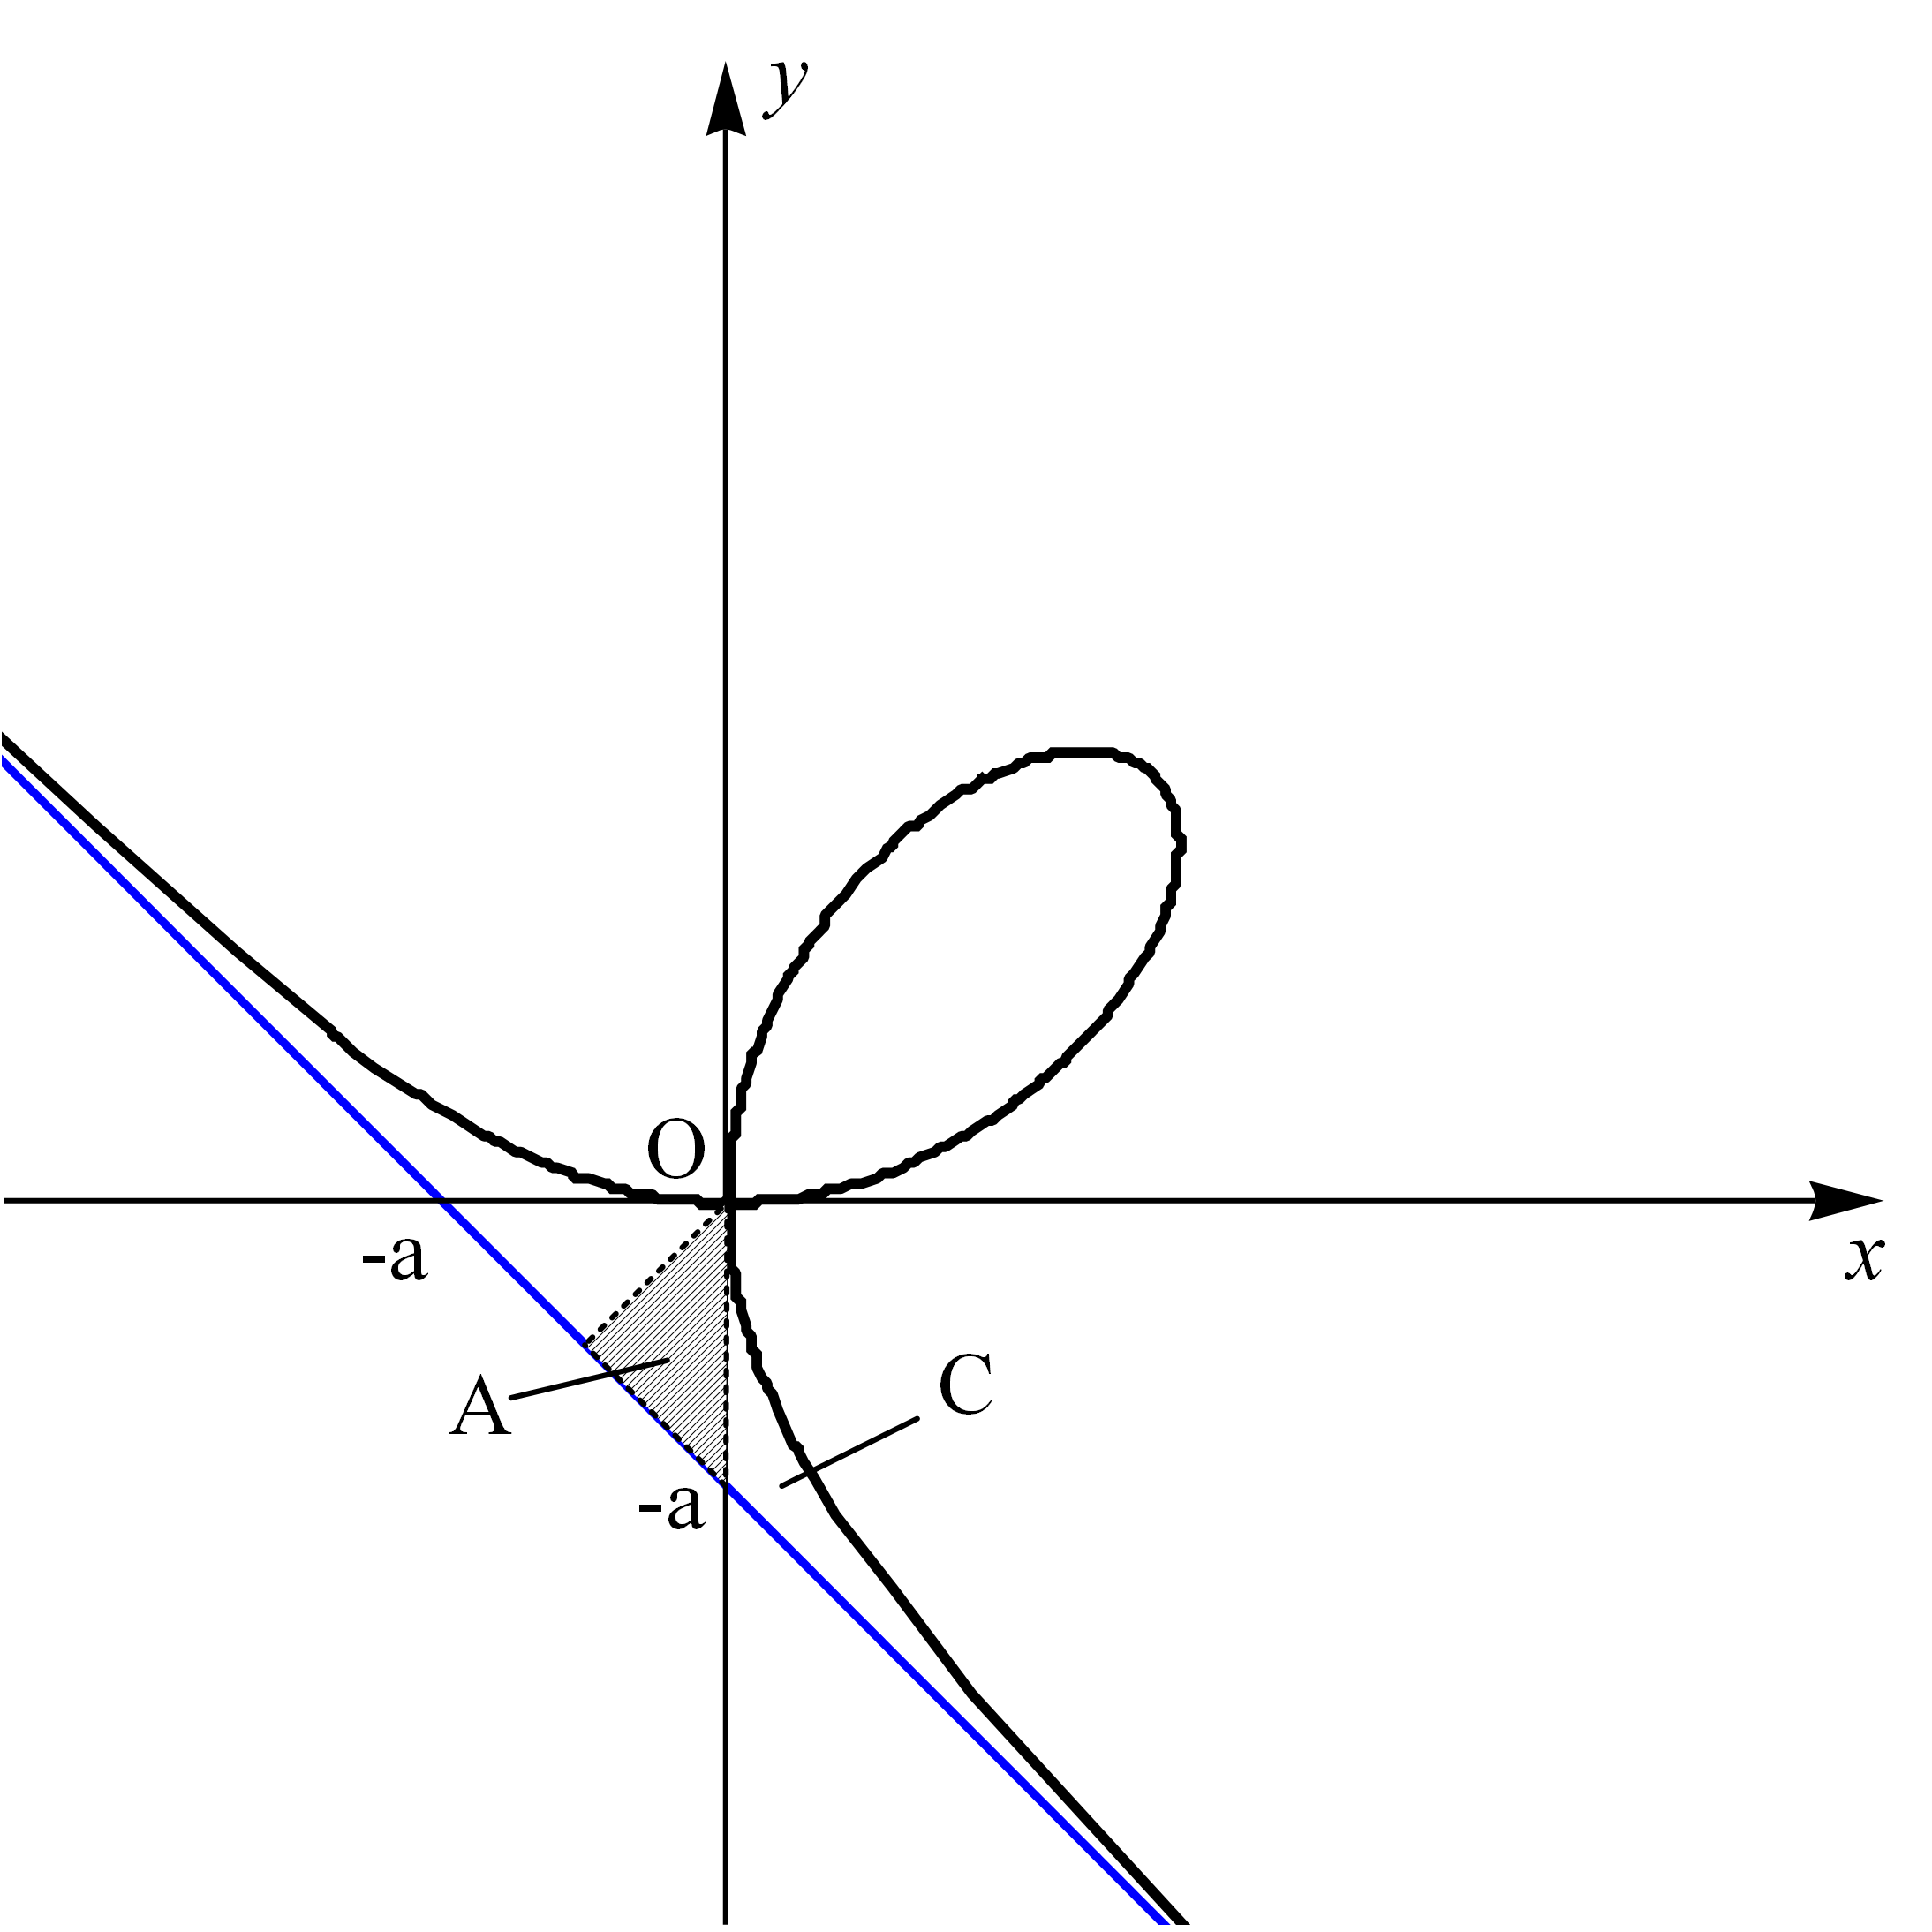
\includegraphics[height=0.4\textheight]{F:/life/2018AutumnTA/Exercises/11CExtra/Fig15.png}
\end{center}
\caption{第7章补充题 15题图示}
\label{15}
\end{figure}

由上图可知$r=r(\theta),0\leq\theta\leq\frac\pi2$是曲线的自闭部分. 

自闭部分的面积为$S_1=\frac12\int_0^{\frac\pi2}r^2(\theta)\mathrm d\theta=\frac12\int_0^{\frac\pi2}\frac{9a^2\sin^2\theta\cos^2\theta}{(\cos^3\theta+\sin^3\theta)^2}\mathrm d\theta\xlongequal[\mathrm dt=\sec^2\theta\mathrm d\theta]{t=\tan\theta}\frac{9a^2}2\int_0^{+\infty}\frac{t^2}{(1+t^3)^2}\mathrm dt\\
=\frac{3a^2}2\int_0^{+\infty}\frac{\mathrm d(1+t^3)}{(1+t^3)^2}=-\frac{3a^2}2\frac1{1+t^3}\Big|_0^{+\infty}=\frac32a^2$.

(2)利用对称性,曲线与渐近线围成的面积为图\ref{15}中A和C两部分面积之和的二倍,

渐近线的参数方程为$r_1(\theta)=-\frac a{\sin\theta+\cos\theta}$,

则C部分的面积$S_C=\frac12\int_{\frac\pi2}^{\frac34\pi}[r_1^2(\theta)-r^2(\theta)]\mathrm d\theta=\frac12\int_{\frac\pi2}^{\frac34\pi}[\frac{a^2}{(\sin\theta+\cos\theta)^2}-\frac{9a^2\sin^2\theta\cos^2\theta}{(\sin^3\theta+\cos^3\theta)^2}]\mathrm d\theta\\
\xlongequal[\mathrm dt=\frac12\sec^2\theta\mathrm d\theta]{t=\tan\theta}\frac12\int_{-\infty}^{-1}[\frac{a^2}{(t+1)^2}-\frac{9a^2t^2}{(t^3+1)^2}]\mathrm dt=\frac12[-\frac{a^2}{t+1}+\frac{3a^2}{t^3+1}]\Big|_{-\infty}^{-1}=\frac12\frac{a^2(2-t)(1+t)}{(1+t)(t^2-t+1)}\Big|_{-\infty}^{-1}=\frac12\frac{a^2(2-t)}{(t^2-t+1)}\Big|_{-\infty}^{-1}\\
=\frac{a^2}2$,

A部分的面积$S_A=\frac14a^2$,

曲线与渐近线围成的面积$S=2(S_A+S_C)=\frac32a^2$.

{\bf【注意:教材答案中$r''(\theta)<0$的结论有误,$r''(\theta)$在$(0,\frac\pi2)$内有正有负.】}
\item设$f(x)\in C[0,1]$,且$f(x)<1$,证明:方程$2x-\int_0^xf(t)\mathrm dt=1$在区间$(0,1)$上有且只有一个根.

证明:令$F(x)=2x-\int_0^xf(t)\mathrm dt-1$

$\because f(x)\in C[0,1]$

$\therefore f(x)\in R[0,1],\int_0^xf(t)\mathrm dt\in C[0,1],F(x)\in C[0,1]$

$\because f(x)<1$

$\therefore F(1)=1-\int_0^1f(t)\mathrm dt>0$

又$\because F(0)=-1<0$

$\therefore\exists\xi\in(0,1),s.t.F(\xi)=0$

$\because F'(x)=2-f(x)>1>0$

$\therefore F(x)$在$[0,1]$上单调增加

$\therefore\xi$唯一,即方程$2x-\int_0^xf(t)\mathrm dt=1$在区间$(0,1)$上有且只有一个根.
\item计算积分$\int_0^{\frac\pi2}\ln(\sin x)\mathrm dx$和$\int_0^\pi\ln(1+\cos x)\mathrm dx$.

解:(1)$I=\int_0^{\frac\pi2}\ln(\sin x)\mathrm dx\xlongequal{x=\frac\pi2-t}\int_{\frac\pi2}^0\ln[\sin(\frac\pi2-t)]\mathrm d(\frac\pi2-t)=\int_0^{\frac\pi2}\ln(\cos x)\mathrm dx$,

$I=\int_0^{\frac\pi2}\ln(\sin x)\mathrm dx\xlongequal{u=\pi-x}\int_\pi^{\frac\pi2}\ln[\sin(\pi-u)]\mathrm d(\pi-u)=\int_{\frac\pi2}^\pi\ln(\sin x)\mathrm dx\\
=\frac12[\int_0^{\frac\pi2}\ln(\sin x)\mathrm dx+\int_{\frac\pi2}^\pi\ln(\sin x)\mathrm dx]=\frac12\int_0^\pi\ln(\sin x)\mathrm dx$,

$2I=\int_0^{\frac\pi2}\ln(\sin x)\mathrm dx+\int_0^{\frac\pi2}\ln(\cos x)\mathrm dx=\int_0^{\frac\pi2}\ln(\sin x\cos x)\mathrm dx$,

$2I+\frac\pi2\ln2=\int_0^{\frac\pi2}\ln(\sin x)\mathrm dx+\int_0^{\frac\pi2}\ln(\cos x)\mathrm dx+\int_0^{\frac\pi2}\ln2\mathrm dx=\int_0^{\frac\pi2}\ln(\sin2x)\mathrm dx\\
=\frac12\int_0^\pi\ln(\sin x)\mathrm dx=I$,

$\therefore\int_0^{\frac\pi2}\ln(\sin x)\mathrm dx=I=-\frac\pi2\ln2$.

(2)$\int_0^\pi\ln(1+\cos x)\mathrm dx\xlongequal{x=2u}\int_0^{\frac\pi2}\ln(1+\cos2u)\mathrm d2u=2\int_0^{\frac\pi2}\ln(1+\cos2x)\mathrm dx\\
=2\int_0^{\frac\pi2}\ln(2\cos^2x)\mathrm dx=2\int_0^{\frac\pi2}\ln2\mathrm dx+2\int_0^{\frac\pi2}\cos x\mathrm dx=\pi\ln2+2I=\pi\ln2-\pi\ln2=0$.
\item设$f(x)$连续,$\varphi(x)=\int_0^1f(xt)\mathrm dt$,且$\lim\limits_{x\rightarrow0}\frac{f(x)}x=A$($A$为常数). 求$\varphi'(x)$且讨论$\varphi'(x)$在$x=0$的连续性.

解:$\varphi(x)=\int_0^1f(xt)\mathrm dt\xlongequal{xt=u}\int_0^xf(u)\mathrm d\frac ux=\frac1x\int_0^xf(u)\mathrm du(x\neq0)$

$\because f(x)$连续且$\lim\limits_{x\rightarrow0}\frac{f(x)}x=A$($A$为常数)

$\therefore f(0)=0$,当$x=0$时,$\varphi(0)=\int_0^1f(0)\mathrm dt=0$

$\therefore\varphi(x)=\begin{cases}
\frac1x\int_0^xf(u)\mathrm du,&x\neq0\\
0,&x=0
\end{cases}$

$\therefore\varphi'(x)=\begin{cases}
-\frac1{x^2}\int_0^xf(u)\mathrm du+\frac1xf(x),&x\neq0\\
\lim\limits_{x\rightarrow0}\frac{\varphi(x)-\varphi(0)}{x-0}=\lim\limits_{x\rightarrow0}\frac{\frac1x\int_0^xf(u)\mathrm du-0}{x-0}=\lim\limits_{x\rightarrow0}\frac{\int_0^xf(u)\mathrm du}{x^2}=\lim\limits_{x\rightarrow0}\frac{f(x)}{2x}=\frac A2,&x=0
\end{cases}$

$\because\lim\limits_{x\rightarrow0}-\frac1{x^2}\int_0^xf(u)\mathrm du=\lim\limits_{x\rightarrow0}-\frac{f(x)}{2x}=-\frac A2$

$\therefore\lim\limits_{x\rightarrow0}\varphi'(x)=\lim\limits_{x\rightarrow0}[-\frac1{x^2}\int_0^xf(u)\mathrm du+\frac1xf(x)]=-\frac A2+A=\frac A2=\varphi'(0)$

故$\varphi'(x)$在$x=0$连续.
\item设$f(x)\in C^2[a,b]$,试证:$\exists\xi\in[a,b]$,使得
\[
\int_a^bf(x)\mathrm dx=(b-a)f(\frac{a+b}2)+\frac1{24}(b-a)^3f''(\xi).
\]
证明:$\because f(x)\in C^2[a,b]$

$\therefore f(x)=f(\frac{a+b}2)+f'(\frac{a+b}2)(x-\frac{a+b}2)+\frac{f''(\eta)}{2!}(x-\frac{a+b}2)^2,\eta$介于$x$和$\frac{a+b}2$之间

$\because f''(\eta)$作为关于$x$的函数在区间$[a,b]$上连续,$g(x)=(x-\frac{a+b}2)^2$在$[a,b]$上可积且非负

$\therefore\exists\xi\in(a,b),s.t.\int_a^b\frac{f''(\eta)}{2!}(x-\frac{a+b}2)^2\mathrm dx=\frac{f''(\xi)}{2!}\int_a^b(x-\frac{a+b}2)^2\mathrm dx=\frac{f''(\xi)}{2!}\frac13(x-\frac{a+b}2)^3\Big|_a^b\\
=\frac1{24}(b-a)^3f''(\xi)$

$\because\int_a^bf'(\frac{a+b}2)(x-\frac{a+b}2)\mathrm dx=f'(\frac{a+b}2)\int_a^b(x-\frac{a+b}2)\mathrm dx=f'(\frac{a+b}2)\frac12(x-\frac{a+b}2)^2\Big|_a^b=0$

$\therefore\int_a^bf(x)\mathrm dx=\int_a^b[f(\frac{a+b}2)+f'(\frac{a+b}2)(x-\frac{a+b}2)+\frac{f''(\eta)}{2!}(x-\frac{a+b}2)^2]\mathrm dx\\
=(b-a)f(\frac{a+b}2)+\frac1{24}(b-a)^3f''(\xi)$.
\end{enumerate}
\end{document}